%
% --- inline annotations
%
\newcommand{\red}[1]{{\color{red}#1}}
\newcommand{\todo}[1]{{\color{red}#1}}
\newcommand{\TODO}[1]{\textbf{\color{red}[TODO: #1]}}
% --- disable by uncommenting  
% \renewcommand{\TODO}[1]{}
% \renewcommand{\todo}[1]{#1}

\usepackage{xcolor}
\usepackage{graphicx}
\usepackage{booktabs}
\usepackage{amsmath} 
\usepackage{amsfonts}
\usepackage{amssymb}
\usepackage{multirow} 
\usepackage{makecell}
\newcommand{\shline}{\Xhline{1.1pt}} % Adjust thickness as desired

\section{Experiments}
\label{sec:experiments}

We present results for supervised video classification and self-supervised masked auto-encoding with frozen representations evaluated on two downstream tasks: video classification and point tracking. To analyse the memory capabilities of our model, we also include a reconstruction task of frames seen in the distant past. Using the same task, we study the generalisation capabilities to longer sequences than seen during training. We follow the ViT scaling configurations and, unless otherwise stated, we use the \textbf{B}ase version for our model for all our experiments. We specify the number of parameters for all models considered in our experiments, and we include in the supplementary material all the training hyperparameters and data augmentations used in all experiments.

\subsection{Supervised video classification}

\par \noindent \textbf{Datasets:}
We use large-scale real-world datasets for the supervised video classification task. Kinetics400~\citep{Carreira_2017_CVPR} contains 241,512 videos\footnote{Kinetics is a dynamic dataset (videos may be removed from
YouTube). Our current version has 241,512 videos, compared to 267,000 videos reported in~\cite{vivit}, so a decrease of almost 10\%, noticeable in the final performance.} across train, validation, and test splits, 10s-long (25fps), spanning 400 classes. This dataset is known to require modelling appearance for successful action recognition. To challenge our model's capability of understanding motion, we also use SSv2 dataset~\citep{goyal2017something}, which contains 220,847 shorter videos (2-6s long), sampled at 12fps, representing 174 classes. This dataset includes actions that differ in finer motion-related details, requiring a deeper temporal understanding, e.g. \textit{pouring something into something} vs \textit{pretending to pour something into something}. 

\par \noindent \textbf{Baselines:}
We use ViViT~\citep{vivit} as our main baseline. We consider the full self-attention version, which patchifies and flattens the entire video, prepends a video class token, then runs self-attention blocks. We also consider the factorised encoder version (ViViT FE), which runs a ViT image model over all the frames, and uses temporal self-attention blocks to integrate the information over time. Finally, we also consider a baseline that uses only LRU recurrent and MLP blocks, configured similar to VideoMamba~\cite{li2024videomambastatespacemodel}, i.e. it does not use self-attention blocks, denoted \textit{PureLRU}. Similar to ViViT, this model first patchifies and flattens the video, prepends a class token, then applies a sequence of recurrent blocks. All baselines use learnt spatio-temporal positional encoding, whereas the proposed \ssm\ uses only spatial positional encoding as the temporal dimension is implicitly modelled through its recurrence.


\par \noindent \textbf{Results:} We include results for training from scratch or using Imagenet pre-trained weights to initialise the weights of the ViT blocks. Figure~\ref{fig:baselines} shows a first comparison between \ssm\ and the above baselines, with all models being trained from scratch on supervised classification on SSv2. We consider the \textbf{S}mall version for all models as the larger \textbf{B}ase version shows stability issues when trained from scratch, as reported in other works as well~\cite{li2024videomambastatespacemodel,vivit}. As expected, the performance on this challenging dataset when training from scratch is far from SOTA, but it clearly shows that the proposed factorisation has superior video modelling capabilities compared to baselines, ViViT-S with full self-attention being the closest competitor. PureLRU's performance is very poor, which is in line with the findings of other works (\eg VideoMamba) who report that bidirectional (non-causal) processing of the input is needed for good performance. 

We report further results comparing against ViViT-B and ViViT-L with full self-attention when using Imagenet pre-trained weights; see Table~\ref{tab:ssv2} for SSv2 results and Table~\ref{tab:kinetics} for Kinetics400 results.
We can observe that our model achieves better performance compared to ViViT baselines on SSv2, but it is slightly below ViViT-L on Kinetics400. This result could reflect the difference between the two datasets mentioned above: outperforming ViViT-L on SSv2 suggests that \ssm\ is superior at modelling motion compared to ViViT, but on Kinetics where the appearance is enough for successful classification, both models are on par. We consider this to be a strong positive result for our model given that it has about 3x less parameters compared to ViViT-L and significantly lower FLOPs count and memory footprint as shown in Figure~\ref{fig:memory}.

\begin{figure}[t]
  \centering
  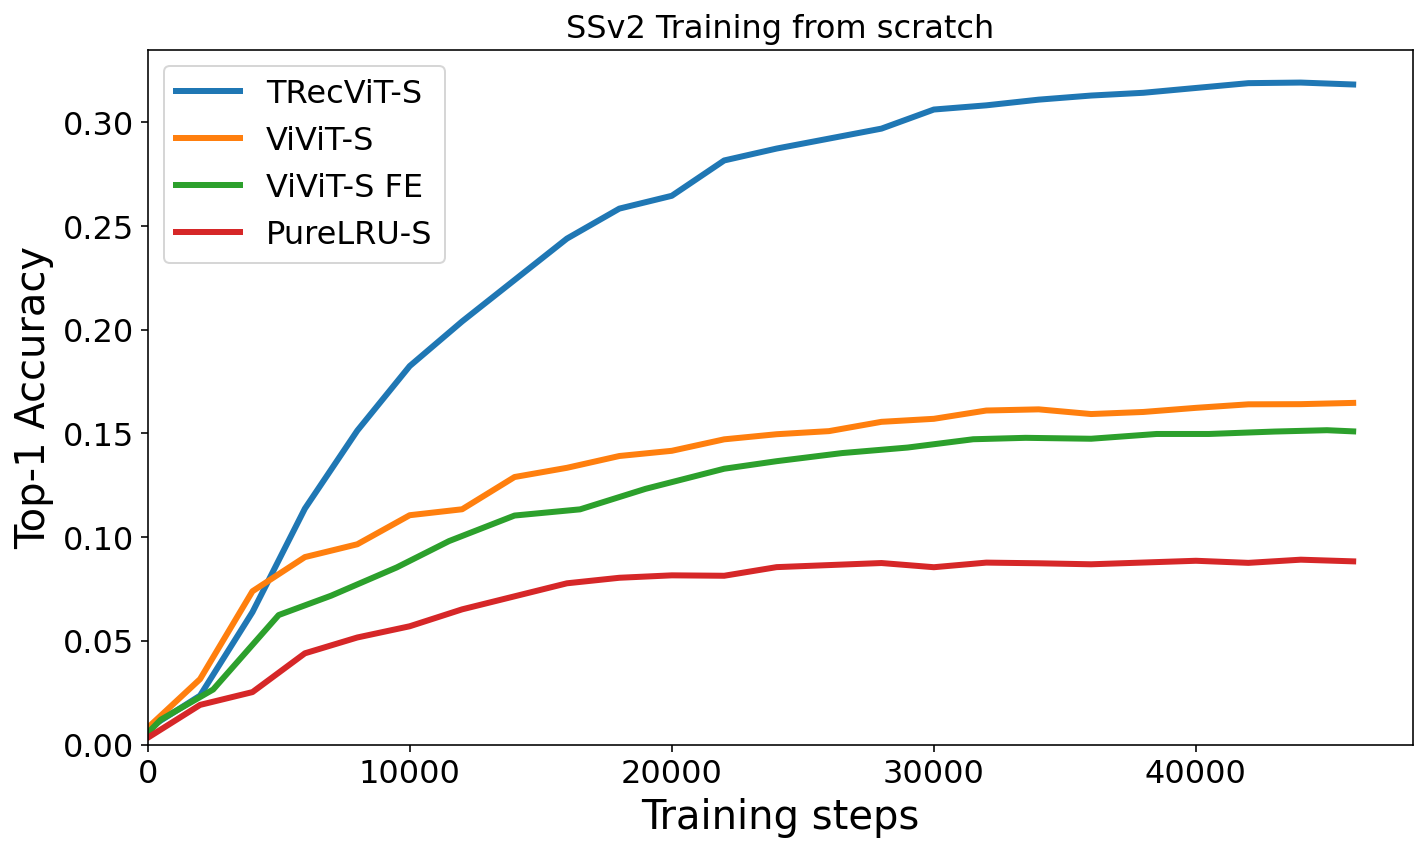
\includegraphics[width=.9\linewidth]{img/scratch.png}
  \caption{\ssm\ compared to baselines on supervised video classification on SSv2 dataset, trained from scratch. The plot shows the evolution of the evaluation accuracy as training progresses.
  }

  \label{fig:baselines}
\end{figure}
 

 \begin{figure*}[h]
  \centering
  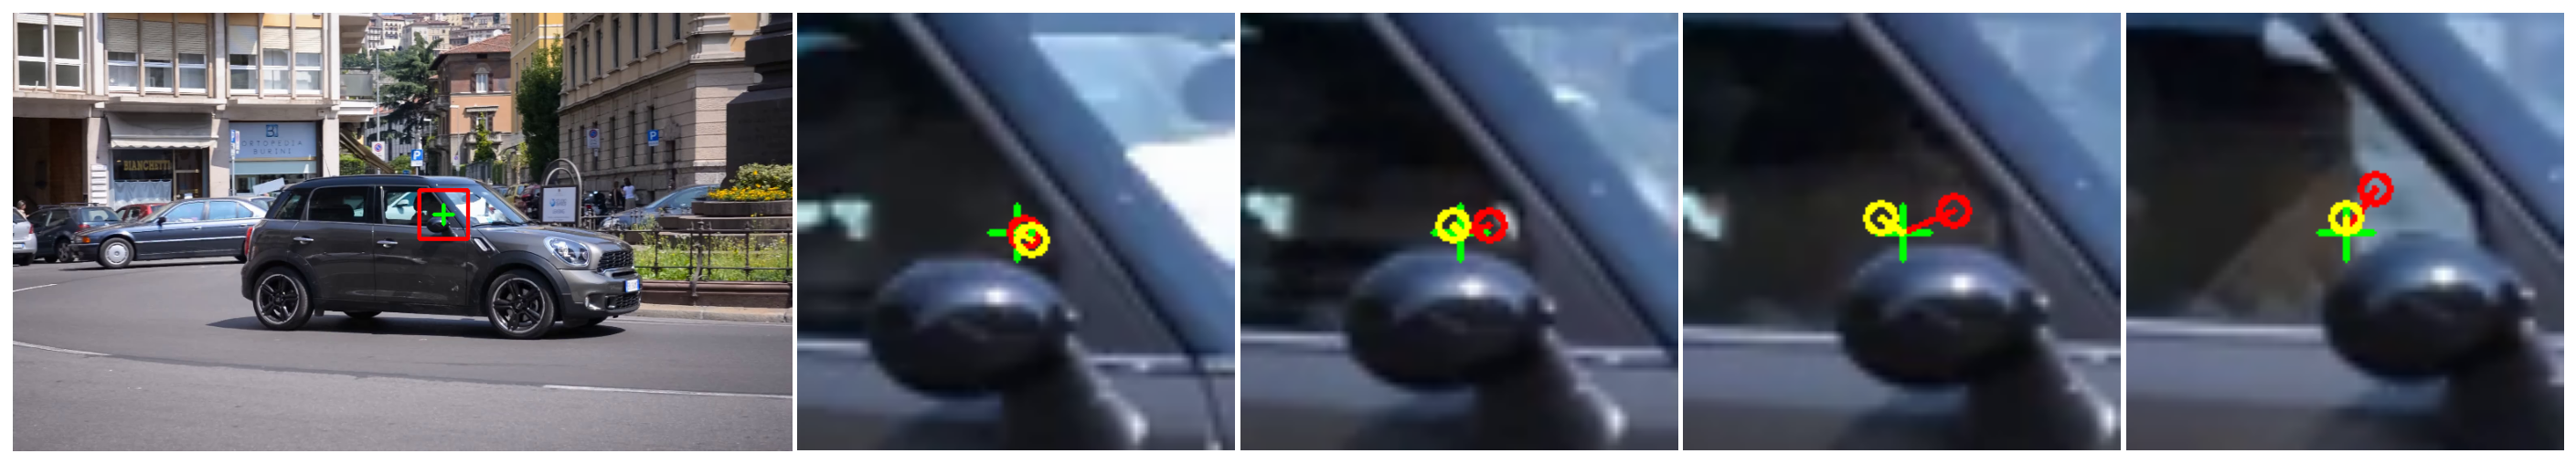
\includegraphics[width=\linewidth]{img/davis.png}
  \caption{Qualitative results obtained by \ssm\ for point tracking on DAVIS dataset compared to VideoMAE. The leftmost image indicates the point to track in the original frame, and the images towards the right show zoom-ins on subsequent frames. Green plus (+) marker indicates the ground truth, yellow circle indicates \ssm's predictions and red circles indicate VideoMAE's predictions.}
  \label{fig:tracking}
\end{figure*}


\begin{table}
    \centering
    \small{
    \begin{tabular}{l|c|c|r}
    \hline
    \textbf{Model} & \textbf{Patch size} & \textbf{Top-1 acc (\%)} & \textbf{\# params} \\
    \hline
    ViViT-B & (2, 16, 16) & 59.1 & 90M \\
    ViViT-L & (2, 16, 16) & 65.9 & 320M \\
    \ssm\ & (1, 16, 16) & \textbf{66.8} & 109M\\
    \hline
    \end{tabular}}
    \caption{Performance of \ssm\ compared to ViViT-B and ViViT-L baselines on SSv2 dataset with all models initialised from Imagenet pre-training. For ViViT-L, we use the result reported by its authors, for ViViT-B we obtained the results internally as they were not reported in the original paper for this dataset.}
    \label{tab:ssv2}
    \end{table}
    
\begin{table}
    \centering
    \small{
    \begin{tabular}{l|c|c|r}
    \hline
    \textbf{Model} & \textbf{Patch size} & \textbf{Top-1 acc (\%)} & \textbf{\# params} \\
    \hline
    ViViT-B & (2, 16, 16) & 78.1 & 90M \\
    ViViT-L & (2, 16, 16) & \textbf{78.7} & 320M \\
    \ssm\ & (1, 16, 16) & 78.4 & 109M\\
    \hline
    \end{tabular}}
    \caption{Performance of \ssm\ compared to ViViT-B and ViViT-L baselines on Kinetics400 dataset, with all models initialised from Imagenet pre-training. For ViViT-B and ViViT-L, we include the result we obtained internally by re-training the model on the current Kinetics400 dataset version; see footnote. In the original paper, the authors reported 80.3\% on Kinetics400 for ViViT-L.}
    \label{tab:kinetics}
    \end{table}

\subsection{Self-supervised masked autoencoding}
\label{sec:mae}
We use Kinetics400 for self-supervised pre-training from scratch and we report results on multiple downstream datasets and tasks by fine-tuning attention readout heads on top of frozen representations. We choose this setup, as opposed to fine-tuning end-to-end, as the  performance in this case more clearly reflects the quality of the pre-trained representations. As mentioned in the previous section, we use a large masking ratio (0.90), which makes pre-training very efficient. We report the number of parameters for every model considered. Note that the number of parameters for \ssm\ is different from the one reported in the previous section due to the addition of the readout heads.

\par \noindent \textbf{Video classification:}  We report video classification accuracy as downstream task using attention readout heads on SSv2 and Kinetics400. We compare the performance against VideoMAE-L~\cite{tong2022videomae} in Table~\ref{tab:selfsup}. Our model obtains slightly better performance on both datasets compared to this strong baseline, despite having almost 3$\times$ less parameters. 

\par \noindent \textbf{Point tracking:} To demonstrate that our model can handle dense(r) tasks as well, we evaluate the same frozen MAE representations for the point tracking task. We use the recurrent architecture in MooG~\cite{steenkiste2024moving} as a readout due to its simplicity. MooG uses light cross-attention layers to process the embeddings of each frame in order, and the readout state is carried over through time. We finetune the MooG readout head using MOVi-E dataset~\cite{movie} as done in popular point tracking works~\cite{DoerschYVG0ACZ23}. We evaluate these fine-tuned representations on two datasets: Perception Test~\citep{patraucean2023perception} and DAVIS dataset~\cite{davis2017} with point tracks extracted in~\cite{doersch2022tapvid}. We report average Jaccard metric~\cite{doersch2022tapvid} for \ssm\ compared with MooG and VideoMAE; see Table~\ref{tab:pt}. \ssm\ obtains better performance on both datasets compared to baselines, which reinforces the observation that our proposed model has strong motion modelling capabilities. We include qualitative results for this task in Figure~\ref{fig:tracking}. We can observe that the results are visibly better compared to VideoMAE. More visualisations are included in the supplementary material.

\begin{table}
    \centering
    \small{
    \begin{tabular}{l|c|c|r}
    \hline
    \textbf{Model} & \textbf{Dataset} & \textbf{Top-1 acc (\%)} & \textbf{\# params} \\
    \hline
    VideoMAE & Kinetics400 & 45.8 & 330M \\
    \ssm\ & Kinetics400 & \textbf{46.0} & 128M\\
    \hline
    \hline
    VideoMAE & SSv2 &  53.7 & 330M \\
    \ssm\ & SSv2 &  \textbf{53.9} & 128M\\
    \hline
    \end{tabular}}
    \caption{Performance of \ssm\ compared to VideoMAE on video classification using frozen MAE representations, pre-trained on Kinetics400.}
    \label{tab:selfsup}
    \end{table}

\begin{table}
    \centering
    \small{
    \begin{tabular}{l|c|c|c|r}
    \hline
    \textbf{Model} & \textbf{Dataset} & \textbf{\# frames} & \textbf{AJ} & \textbf{\# params} \\
    \hline
    MooG & DAVIS & 8 & 0.687 & 35M \\
    VideoMAE & DAVIS & 8 & 0.703 & 330M \\
    \ssm\ & DAVIS & 8 & \textbf{0.706} & 128M\\
    
    \hline
    \hline
    MooG & Perception Test & 16 & 0.760 & 46.5M \\
    VideoMAE & Perception Test & 16 & 0.761 & 330M \\
    \ssm\ & Perception Test & 16 & \textbf{0.783} & 128M\\
    \hline
    \end{tabular}}
    \caption{Performance of \ssm\ compared to baselines on point tracking task on DAVIS and Perception Test datasets. All models use frozen representations evaluated using the readout head from MooG.}
    \label{tab:pt}
    \end{table}

\begin{figure*}[h]
  \centering
  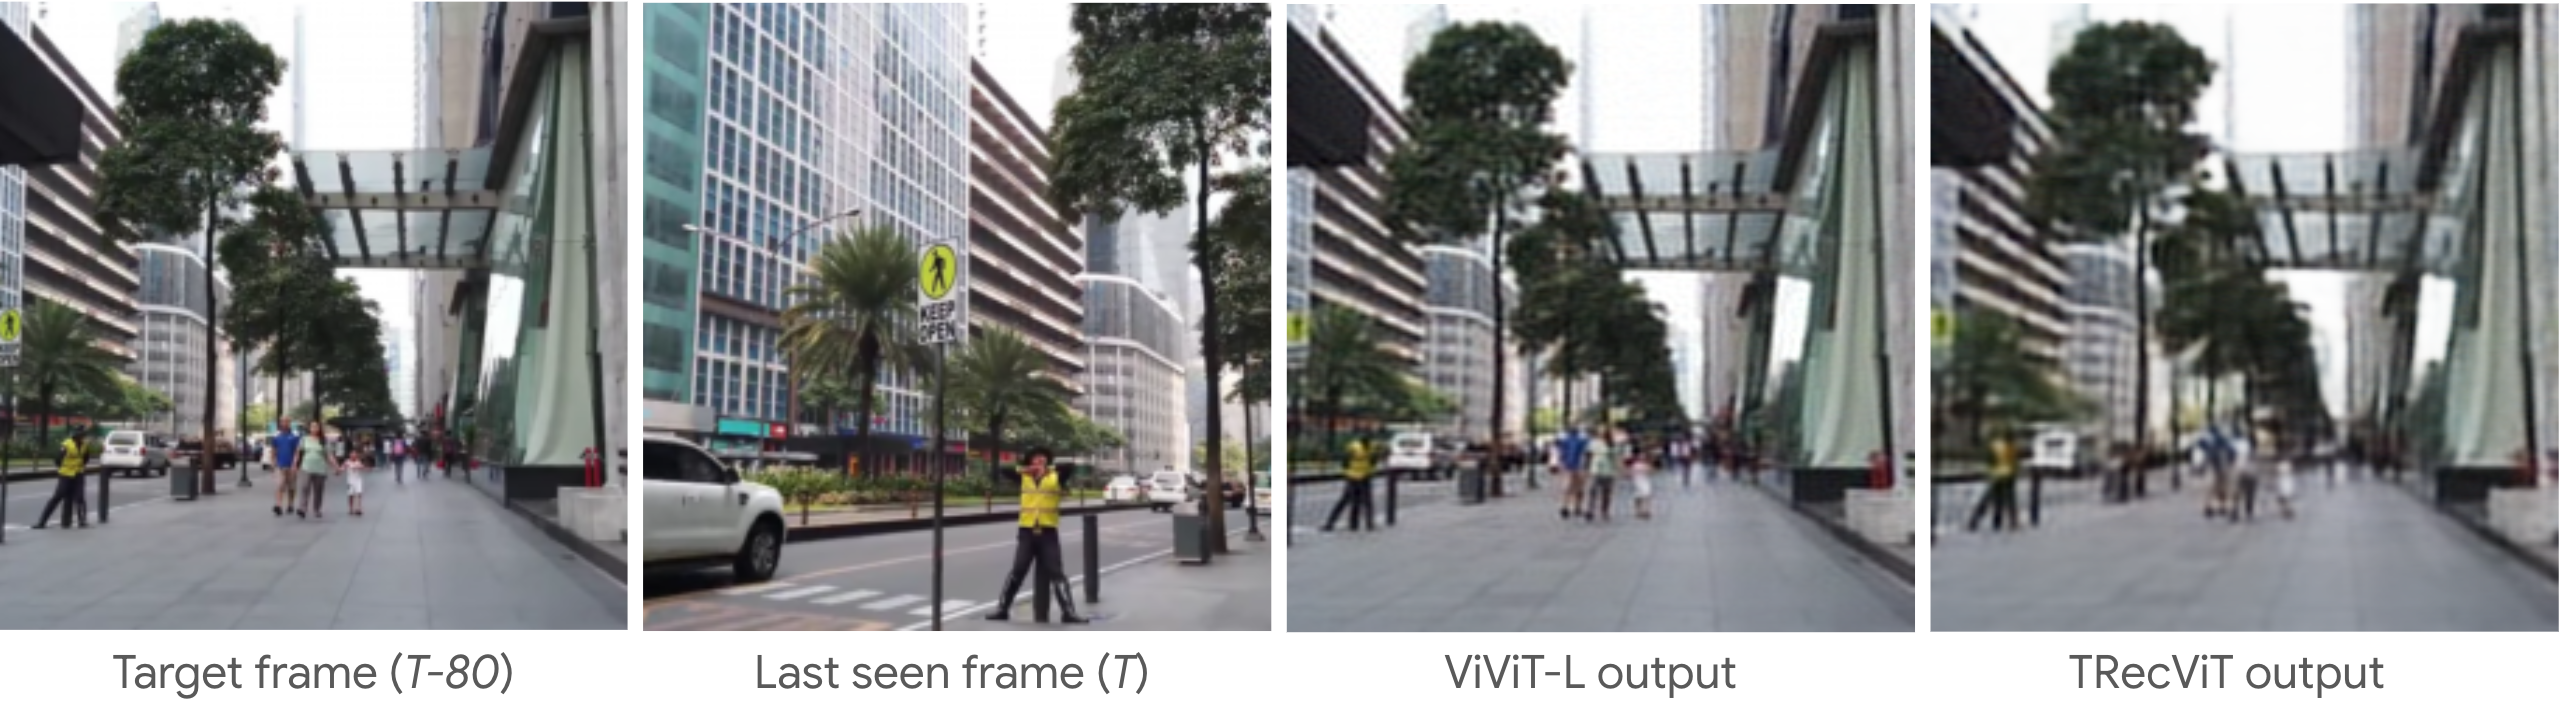
\includegraphics[width=\linewidth]{img/wtlong.png}
  \caption{Qualitative results obtained by \ssm\ on the dense memorisation task compared to ViViT-L. Both models are trained using Imagenet pre-trained weights, on video sequences of $T=64$ frames and they reconstruct the $(T-48)^\text{th}$ frame.}
  \label{fig:wt}
\end{figure*}

\begin{figure}[t]
\centering
\begin{subfigure}{0.48\linewidth}
    \centering
    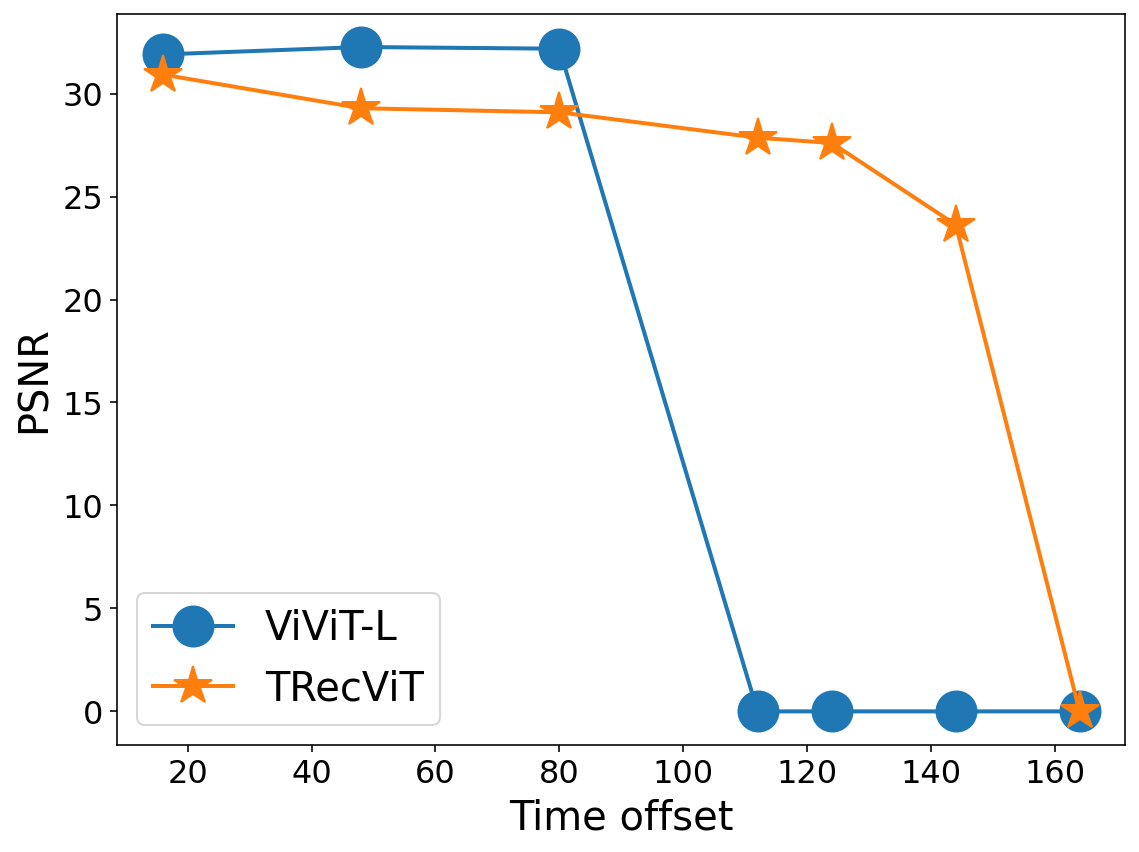
\includegraphics[width=\textwidth]{img/psnr.png}
    \caption{PSNR comparison}
\end{subfigure}%
\hfill
\begin{subfigure}{0.48\linewidth}
    \centering
    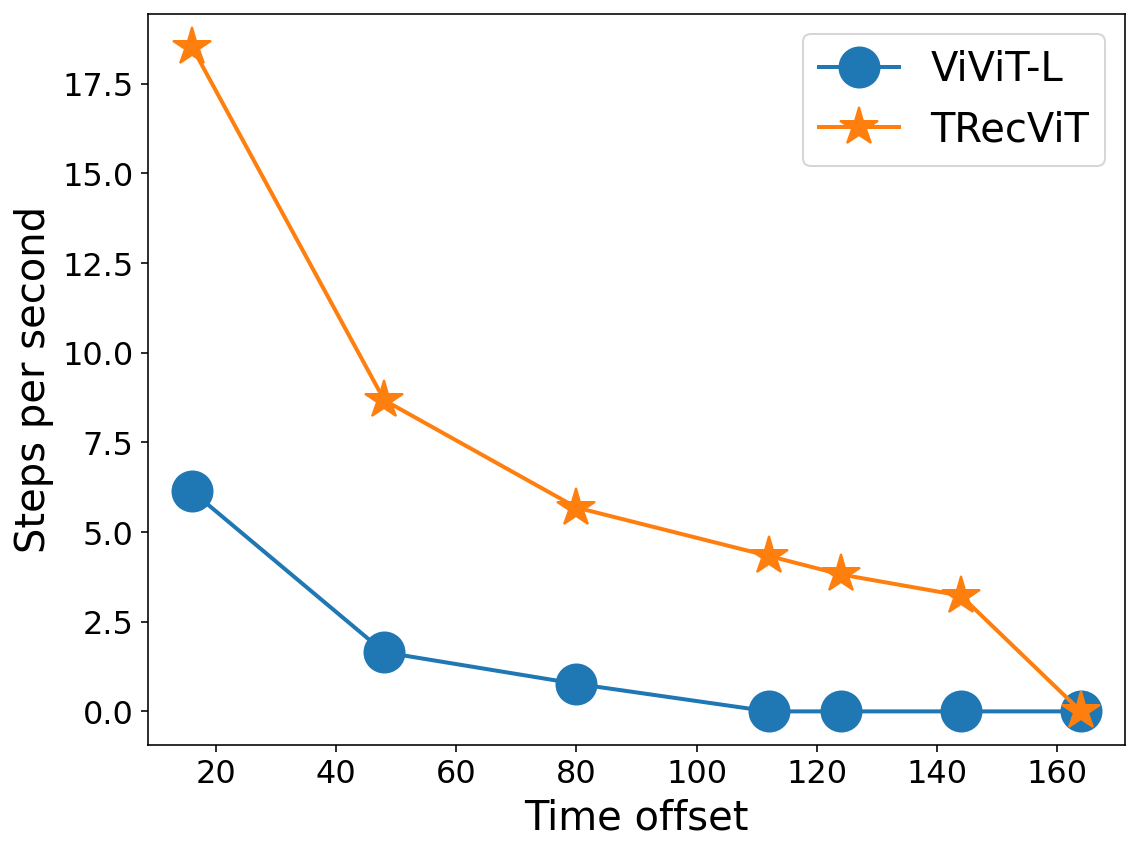
\includegraphics[width=\textwidth]{img/sps.png} 
    \caption{Steps-per-second comparison}
\end{subfigure}
\caption{Long video memorisation task. At time $T$, the model has to reconstruct the $(T-k)^\text{th}$ frame seen in the past. The plots show PSNR and throughput (steps-per-second) for increasing time offset $k$. For both models, the data points with $0$ value on the $y$-axis correspond to OOM.
}
\label{fig:psnr}
\end{figure}

\subsection{Long video memorisation task}
\label{sec:longtask}

Transformer models for language are known to be excellent at retrieving information from context, as they cache the keys and values for the entire history. On the other hand, LRUs / SSMs and RNNs in general struggle with such \emph{needle-in-the-haystack} style tasks as they need to perform the retrieval based on the compressed history kept in their recurrent state~\cite{jelassi2024repeat, de2024griffinmixinggatedlinear}. 
We are interested in studying this aspect in the video domain as well. We set up a simple reconstruction task where the model has to remember the frame seen at a given time-step in the past. For our analysis, we run multiple experiments where the model is tasked to reconstruct the $(T-k)^{\text{th}}$ frame from the past, with increasing value for $k\in\{16, 48, 80, 112, 144, 164\}$ frames. We employ Walking Tours dataset~\cite{venkataramanan2023imagenet}, which contains hour-long videos, and the scenery changes constantly, hence we are guaranteed that the video frames seen most recently will be very different compared to the frames seen earlier on. We scale the videos to $224\times224$ pixels. Again, we adopt ViViT-L as baseline, and we train both models using Imagenet pretrained weights. For ViViT-L, we keep all the outputs from all $T$ time steps and apply temporal pooling and a $1\times1$ convolution to get the expected shape for the reconstructed frame. For \ssm, we simply keep the output of the last layer at time step $T$ and reshape it to the expected shape. We show quantitative and qualitative results respectively in Figures~\ref{fig:psnr} and~\ref{fig:wt}. We can observe that there is a performance--efficiency trade-off at play for \ssm: its performance is slightly below ViViT's for shorter memory spans (16, 48, 80), but its efficiency (steps-per-second) is significantly higher. However, beyond 80 frames, ViViT-L goes out of memory, whilst \ssm\ continues to give decent results up to 144 frames, going out of memory towards 164 frames. Figure~\ref{fig:wt} shows qualitative results compared to the baseline for the case where the models have to remember the frame seen at $T-48$ in the past. We can observe that the quality of ViViT-L's reconstruction is good. For \ssm, whilst the overall structure (encoded in lower frequencies) is correct, it struggles to remember the high-frequency content of the image. This is to be expected due to the compression happening in the recurrent state of the model. However, given how different the last seen frame is from the target frame, we consider this to be a very promising result that warrants further investigation into the memorisation capabilities of our model, which we leave as future work.

\subsection{Generalisation to longer sequences}
\label{sec:gentask}

Using the same task as above, we analyse the generalisation capabilities to sequences longer than those used during training. Specifically, we train the models with sequences of length $T=64$ frames to reconstruct the $T-48$ frame, and evaluate them on longer sequences $T=96$ to reconstruct the same frame. The \ssm\ model can run on longer sequences without any modification. For the ViViT model, we need to adapt the positional encoding to accommodate longer sequences. We use interpolation to nearest neighbour to obtain the desired length; cubic interpolation led to worse results. The performance of \ssm\ degrades slightly, with PSNR going down from 29.3 (when evaluated on the same sequence length as in training $T=64$) to 26.4 when evaluated with $T=96$ frame sequences. ViViT's PSNR, however, drops significantly, from 32.3 when evaluated on the same sequence length, to 15.1 when evaluated on longer sequences. We include qualitative examples in Figure~\ref{fig:gentask} where we can observe that ViViT's output contains stronger artefacts compared to \ssm. 

\begin{figure}[h]
  \centering
  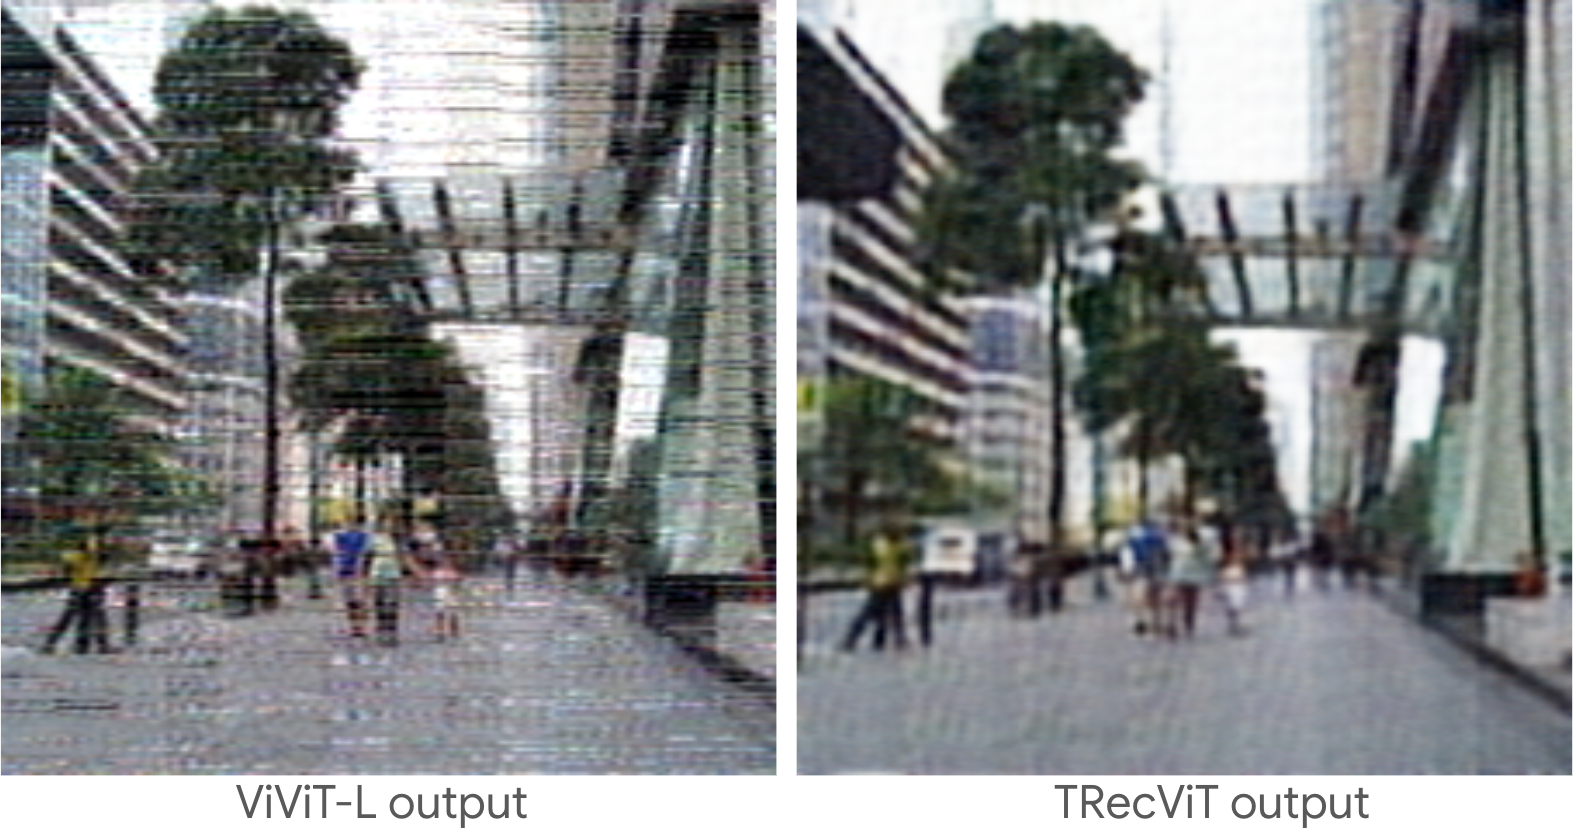
\includegraphics[width=\linewidth]{img/genlong.png}
  \caption{Generalisation to longer sequences. Both models are trained using Imagenet pre-trained weights, on video sequences of $T=64$ frames to reconstruct the $(T-48)^\text{th}$ frame; during evaluation, the models receive sequences of $T=96$ frames.}
  \label{fig:gentask}
\end{figure}
